\documentclass[a4paper]{article}

\usepackage[fontset=fandol]{ctex}
\usepackage{amsmath, amssymb}
\usepackage{graphicx}
\usepackage[margin=2.4cm]{geometry}
\usepackage[most]{tcolorbox}
\usepackage{hyperref}
\usepackage{booktabs}
\usepackage{float}
\usepackage{enumitem}

\newtcolorbox{knowledgebox}[1]{
    enhanced, colback=blue!5!white, colframe=blue!75!black, colbacktitle=blue!75!black,
    coltitle=white, fonttitle=\bfseries, title=#1, attach boxed title to top left={yshift=-2mm, xshift=2mm},
    boxrule=1pt, sharp corners
}

\newtcolorbox{importantbox}[1]{
    enhanced, colback=yellow!10!white, colframe=yellow!80!black, colbacktitle=yellow!80!black,
    coltitle=black, fonttitle=\bfseries, title=#1, sharp corners
}

\newtcolorbox{warningbox}[1]{
    enhanced, colback=red!5!white, colframe=red!75!black, colbacktitle=red!75!black,
    coltitle=white, fonttitle=\bfseries, title=#1, sharp corners
}

\newcommand{\notetitle}{CS294/194-196 第 12 讲：具身自治体、交互与学习}
\newcommand{\noteauthors}{Codex 基于 Peter Stone 讲座视频与官方 readings 重写}
\newcommand{\notedate}{2026-04-16}
\newcommand{\videourl}{https://www.youtube.com/watch?v=iDhzzugMOLA}
\newcommand{\videocoverpath}{../../raw/12_iDhzzugMOLA/12_iDhzzugMOLA.jpg}

\begin{document}

\begin{titlepage}
\centering
{\Large 课程讲义\par}
\vspace{1.2cm}
{\huge\bfseries \notetitle\par}
\vspace{0.8cm}
{\large \noteauthors\par}
\vspace{0.3cm}
{\large \notedate\par}
\vspace{1.2cm}
\includegraphics[width=0.82\textwidth,height=0.45\textheight,keepaspectratio]{\videocoverpath}\par
\vfill
\begin{tcolorbox}[width=0.9\textwidth, colback=black!2!white, colframe=black!60, sharp corners]
\textbf{课程}：UCB CS294/194-196 Agentic AI（Fall 2025）\par
\textbf{讲次}：Autonomous Agents: Embodiment, Interaction, and Learning\par
\textbf{主讲}：Peter Stone, UT Austin / Sony AI\par
\textbf{说明}：官方课程页未提供 slides，本章依据视频、字幕与官方 readings 做 best effort 教材化重建。\par
\textbf{视频}：\href{\videourl}{\nolinkurl{\videourl}}
\end{tcolorbox}
\end{titlepage}

\tableofcontents
\newpage

\section{为什么要把“embodiment”重新放回 agent 讨论中心}
Peter Stone 一开场就把这讲和前面几讲区分开了：课程前半段已经覆盖了 learning、reasoning、multi-agent 和 scientific discovery，但对 \textbf{embodiment} 的讨论还不够。这里的 embodiment 不是抽象的“把 agent 放到世界里”，而是非常具体地指向 robots，包括 physical robots 与 simulated robots。

这讲最重要的第一个判断是：\textbf{all robots are agents, but not all agents are robots。} 这句话把 agent 与 robot 的关系说得很清楚。agent 是更一般的概念，只要系统通过 sensors 和 effectors 与环境形成持续闭环，它就是 agent；而 robot 则是在此基础上进一步要求与 physical world 发生真实交互的特例。

\subsection{本章小结}
把 embodiment 放回 agent 主线，意味着课程不再把 agent 仅仅理解成浏览器、终端和 API 上的数字执行体，而是把它扩展到物理环境中的自治系统。

\section{什么叫 autonomous agent：传感、决策与执行的连续闭环}
这讲给出的定义非常经典：an agent is an intelligent system that interacts with the environment through sensors and effectors。Peter Stone 特别强调 autonomous 的含义在于连续闭环，而不是一轮一轮被外部调用。换句话说，agent 不是“等一个 prompt 再给一个 response”，而是持续接收环境输入、形成内部状态、输出动作，并让这些动作影响下一轮感知。

\begin{figure}[H]
\centering
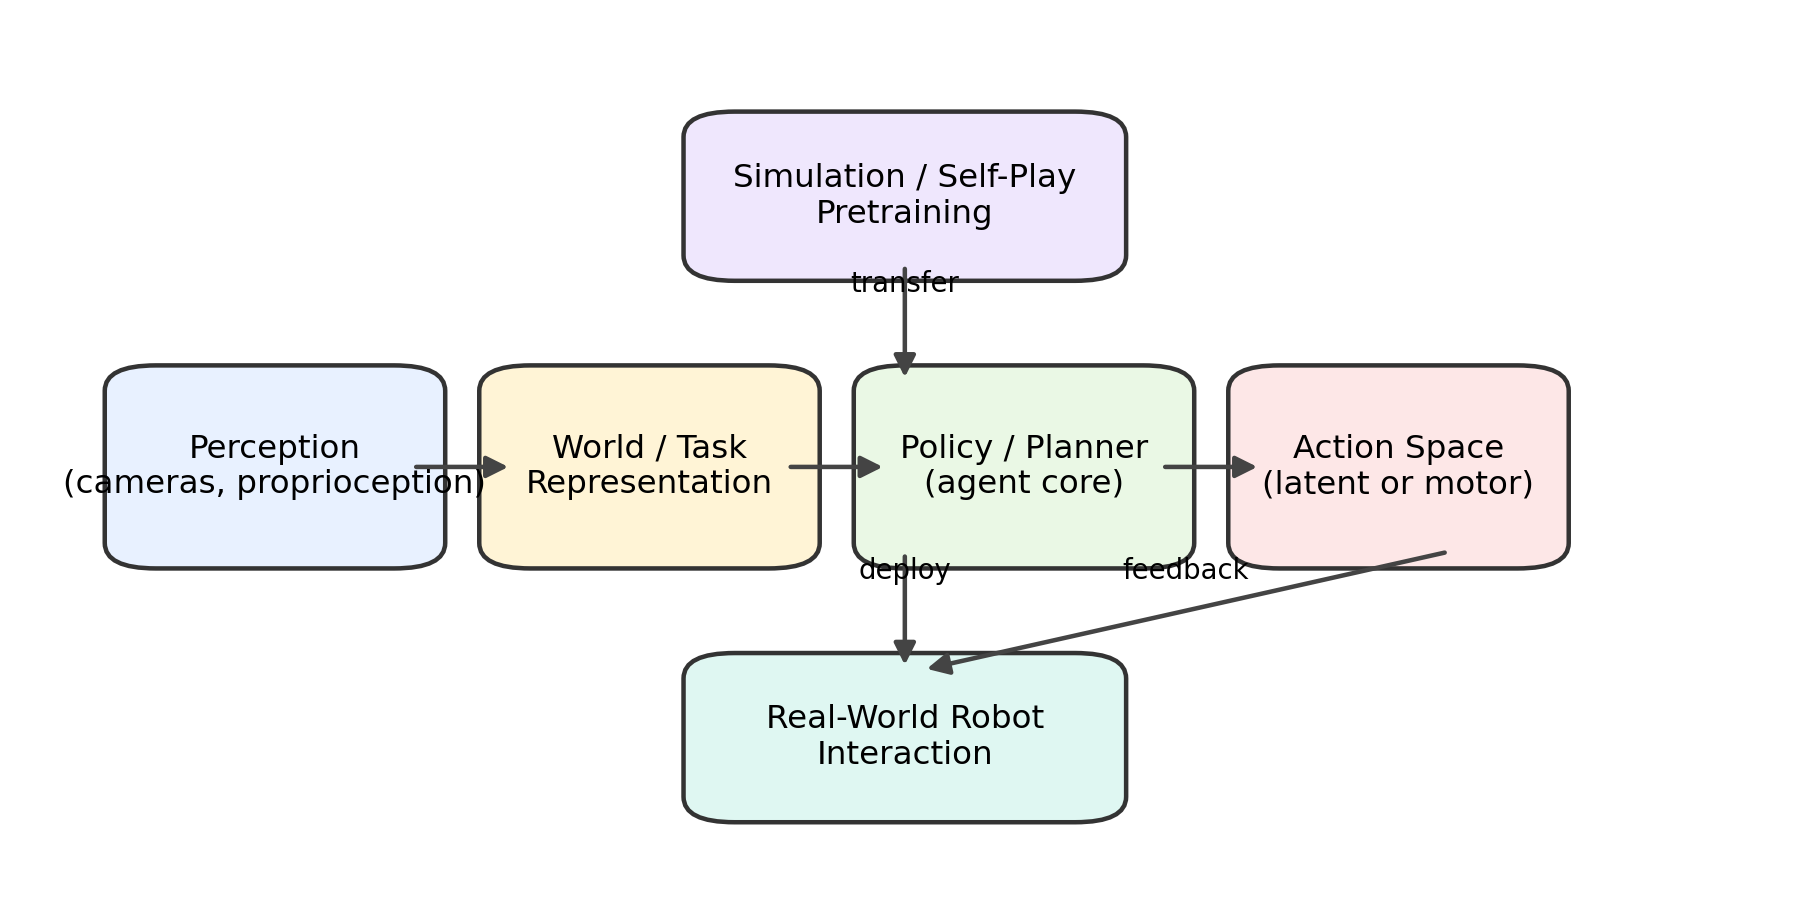
\includegraphics[width=0.88\textwidth]{figures/embodied_agent_stack.png}
\caption{具身自治体的最小闭环：感知、世界/任务表示、策略与规划、动作空间，以及 simulation-to-real 的迁移路径。}
\end{figure}

一旦把定义写成连续闭环，很多看似只是 robotics 里的问题，立刻就变成了 agent 的核心问题。例如：
\begin{itemize}[leftmargin=1.5em]
\item 环境观测是不完整且有噪声的；
\item 行动会改变未来观测；
\item 奖励、任务目标与安全约束常常不是一次性给定；
\item 学习必须和 interaction 紧密耦合。
\end{itemize}

\begin{knowledgebox}{为什么 robotics 会让 agent 定义更清楚}
在浏览器或代码环境里，agent 的 effectors 可能被误看成“只是 API 调用”；在机器人环境里，effectors 直接作用于物理世界，因此 perception--decision--action loop 的本质会被看得更清楚。
\end{knowledgebox}

\subsection{本章小结}
这讲把 autonomous agent 定义重新校准成一个持续闭环系统。这种定义对数字 agent 和物理 robot 同样成立，只是后者把不确定性和安全代价放大了。

\section{从 robot soccer 到 humanoids：多智能体与具身学习的长期路线}
Peter Stone 明确把自己长期的研究线索摆出来：robot soccer、多机器人协作、reinforcement learning、再到 humanoid robots。这条线索的意义，不是罗列历史案例，而是说明具身 agent 的研究从来都不是单机控制问题，而是长期与多智能体、交互学习和真实系统约束绑在一起的。

RoboCup 之所以在这讲里占重要位置，是因为它同时包含 perception、decision making、multi-agent coordination 和 long-horizon task structure。它既是 robotics benchmark，也是 agent benchmark。讲者想借此说明：即便在 LLM 时代，多智能体与具身性也不是分离的话题，而是常常同时出现。

\subsection{为什么 humanoids 让问题进一步升级}
从 AIBO 到 humanoids，并不是“同样问题换个外形”，而是控制维度、感知难度、协作复杂度和安全风险都显著上升。humanoid robots 不仅要做 locomotion，还可能要 manipulation、navigation、human interaction 与长期任务执行。也因此，agent 的设计不再只是 policy 的事情，而是必须同时处理 action abstraction、state representation 和 real-world robustness。

\subsection{本章小结}
robot soccer 和 humanoids 说明，具身 agent 的难点是组合性的：感知、控制、协作和环境不确定性一起出现，不能被拆成互不相干的小问题。

\section{为什么 simulation 和 representation learning 变成关键}
这讲虽然没有官方 slides，但 transcript 和 readings 的组合给出了非常清晰的一条技术路线：\textbf{要做现实世界 robot agents，就必须把 simulation、representation learning 和 real-world adaptation 结合起来。}

补充 reading `Outracing Champion Gran Turismo Drivers with Deep Reinforcement Learning` 强调的是大规模模拟环境、自博弈（self-play）和高度结构化的 reward / evaluation 如何推动复杂技能习得。它虽然是赛车场景，但对这门课的真正启示是：当 environment 足够 rich 且 evaluation 足够清晰时，agent 能通过长期 interaction 学出远超模仿学习的策略。

另一篇 reading `SLAC: Simulation-Pretrained Latent Action Space for Whole-Body Real-World RL` 则把问题推进到更符合 2025 agent 叙事的方向：如何先在 simulation 中预训练 latent action space，再迁移到 real-world embodied RL。它的意义在于：\textbf{行动空间本身可以被学习和压缩。} 对具身 agent 来说，这和 tool abstraction 在数字 agent 里的角色非常类似，都是在降低高维原始动作空间的复杂度。

\begin{importantbox}{这讲与前面 software / web agents 的对应关系}
数字 agent 会抽象 tools 与 workflows，具身 agent 会抽象动作空间与交互接口。两者虽然环境不同，但核心工程动作相似：都在为复杂行动寻找更稳定、更可学习的中间表示。
\end{importantbox}

\subsection{本章小结}
simulation、representation 与 action abstraction 并不是 robotics 里的配套细节，而是让具身 agent 真正可训练、可迁移、可部署的核心支柱。

\section{LLM agent 课程为什么需要 robotics 这一讲}
如果这门课只讲 software agents，很容易让人把 agent 理解成“会调工具的大模型”。Peter Stone 这讲的真正价值，是把 agent 概念重新拉回环境交互、长期学习与 embodied action 的一般形式。也就是说，LLM agent 只是 agent family 的一个分支，而不是定义本身。

从课程结构上看，这一讲至少补了三件事。第一，它提醒我们 memory 和 planning 不只出现在语言链条里，也出现在 physical interaction loop 里。第二，它让 evaluation 问题更难，因为 real-world task success 往往更昂贵、更慢、更难自动验证。第三，它把 safety 的 stakes 提前抬高：一旦动作进入 physical world，错误就不再只是错误文本，而可能是系统级事故。

\begin{warningbox}{为什么不能把具身 agent 当作“以后再说”的外延问题}
如果 agent 课程完全忽略 embodiment，就会默认 environment 永远是可回滚、低成本、数字化的。这会让很多 planning、memory、evaluation 和 safety 讨论失真。
\end{warningbox}

\subsection{本章小结}
这一讲把 agent 从语言和软件环境重新拓展到物理环境，迫使我们重新理解 autonomy、learning、evaluation 和 safety 的含义。

\section{总结与延伸}
这讲最值得带走的结论有四点。

第一，\textbf{autonomous agent 的一般定义是持续的感知--决策--执行闭环，而不是单轮调用。}

第二，\textbf{robot 是具身 agent 的典型形态，它把 environment interaction 的本质放大得最清楚。}

第三，\textbf{simulation、representation learning 和 action abstraction 是具身 agent 的核心方法，而不是辅助技巧。}

第四，\textbf{robotics 之所以重要，不是因为它离 LLM 更远，而是因为它让我们更清楚地看到 agent 概念的真实边界。}

\subsection{拓展阅读}
\begin{itemize}[leftmargin=1.5em]
\item \emph{Outracing Champion Gran Turismo Drivers with Deep Reinforcement Learning}
\item \emph{SLAC: Simulation-Pretrained Latent Action Space for Whole-Body Real-World RL}
\end{itemize}

\subsection{本章小结}
Lecture 12 的意义在于把 agent 重新定义成一般性的自治交互系统。这样看完整门课时，software agents、scientific agents 与 embodied agents 才会被放进同一张地图里。

\end{document}
